\chapter{Analýza problematiky detekce pádu}
\label{chap:Goal}

V této kapitole stanovíme, co je přesně naším cílem, a zamyslíme se, jak k
našemu problému přistoupit.

Naším úkolem bude v reálném čase z videostreamu detekovat pád osoby. Pád osoby
definujeme jako náhle, neúmyslné klesnutí těla z výškové pozice (např. stání,
chůze nebo sezení) na zem nebo jinou nižší úroveň, přičemž tato osoba nemá
kontrolu nad tímto pohybem. Samozřejmě nejsme vždy schopni úplně dobře
rozeznat, zda se nejedná o úmyslné klesnutí, např. prudké lehnutí.

Dle některých definic (zejména ve zdravotnictví) se o pád nejedná, pokud jde o
důsledek závažné vnitřní příhody (např. mrtvice). V našem případě toto
nerozlišujeme, naopak chceme detekovat jak pády v důsledku ztráty rovnováhy či
vlivem vnějších faktorů (např. zakopnutí, převrácení těžkým předmětem), tak
pády v důsledku akutních události vlivem zdravotních problémů, jako jsou např.
mrtvice, záchvaty, mdloby či jiné důvody ztráty vědomí.

\section{Návrh řešení}

Cílem této práce je navrhnout algoritmus, který bude detekovat, zda je ve
vstupní sekvenci snímku některá osoba, jejíž pozice je klasifikována jako pád.
Hlavním cílem výsledného programu bude alarmovat příslušného pracovníka, pokud
osoba upadne.

Alarmovat budeme až, pokud osoba zůstane v ležící pozici. To nám dá možnost
odfiltrovat falešné alarmy v případě sehnutí či pokud bude osoba špatně
viditelná a algoritmus tak na okamžik špatně vyhodnotí její pohyb. Tímto
postprocesingem se ale teď nebudeme zabývat, spíše se zaměříme na samotnou
klasifikaci pozice.

Stejně jako u detekce objektů, viz \ref{sec:obj_det}, bychom mohli i pro
detekci pádu vytvořit vhodnou konvoluční síť, která by přímo z obrázku
definovala, zda se jedná o pád nebo ne. U detekce se už dnes sice s ohledem na
pokrok hardwaru tento přístup používá, nicméně se jedná o velmi náročný úkol,
který vyžaduje rozsáhlou optimalizaci, pokročilou architekturu a velké množství
trénovacích dat. Nicméně, pokud by se podařilo takovouto síť natrénovat, mohla
by lépe detekovat některé situace např. podle výrazu tváře.

V našem případě tedy budeme v prvním kroku pomocí vhodné předtrénované
neuronové sítě detekovat pozici osoby ve formě klíčových bodů, tuto část
nazvěme \textit{detekční algoritmus}. Na základě těchto bodů pak další
neuronová síť vyhodnotí, zda se jedná o pád, tuto část nazvěme
\textit{klasifikační algoritmus}. To úlohu velice zjednoduší, jelikož místo
analyzování tisíců pixelů, budeme analyzovat pár desítek klíčových bodů. Další
výhodou je, že u takového postupu jsme schopní použít techniky, kdy sledujeme
změny pózy v čase, což by bylo mnohem složitější s jednofázovou konvoluční
síti.

Detekční algoritmus dostane na vstup celý snímek a může detekovat několik osob.
Klasifikační algoritmus ale bude zpracovávat každou osobu, resp. její pózu,
zvlášť.

Další alternativou by mohlo být pouze detekovat osoby jako objekty, a na
základě jejich bounding boxů určit, zda se jedná o pád. Tento postup by byl
jednodušší na dvou úrovních. Jednak je detekce objektů méně náročná úloha než
detekce pózy, jednak bychom ve druhé fázi analyzovali pouze několik parametrů
bounding boxu (rozměry a velikost) oproti pár desítkám klíčových bodů. Nicméně,
pokud se nad tím zamyslíme, ne vždy vypovídají parametry bounding boxů o pozici
člověka. Tento postup by tak pravděpodobně vedl k mnohem méně přesnému
výsledku, než analýza klíčových bodů, kdy může síť analyzovat takové vzorce
jako je např. délka končetin v pohledu či úhel mezi nimi.

Nyní se podíváme, jak budeme pracovat s daty, zejména při trénování, v další
kapitole pak bude rozebraná problematika detekce pózy a bude zvolen algoritmus
pro detekci klíčových bodů. Dále se pak budeme zabývat vývojem modelu
detekujícího pád na základě těchto klíčových bodů.

\section{Trénovací datasety}
\label{sec:TrainingData}

Pro trénování našeho modelu jsme použili necelých 150 krátkých (1 až 15 sekund)
videí ze dvou zdrojů. Prvním je dataset CAUCAFall vytvořený právě pro práci s
pády osob \cite{caucafall}. Tento dataset obsahuje 100 nahrávek simulovaných
pádu v různých světelných podmínkách, s různými osobami. Zahrnují širokou škálu
scénářů, jednak pro různé druhy pádů (v různých směrech či z židle), jednak pro
situace podobné pádu, jako je kleknutí či, sehnutí se, jednak běžné činnosti
jako chůze či sednutí. Poměr videí s úpadkem a bez je 50/50.

Dalším zdrojem pro trénovací data je YouTube video tvůrce Kevina Parryho
\textit{50 Ways to Fall}. Ve videu autor pády v různých scénářích, jako je
zakopnutí, omdlení či poražení elektrickým proudem. Vzhledem k zabavné povaze
videa jsme některé scénáře vypustili, nakonec jsme použili 45 videí. Zde prakticky všechny videa obsahují pád, v některých se ale postava vrátí do normálního stavu (např. kotrmelec).

\begin{figure}[]
    \centering
    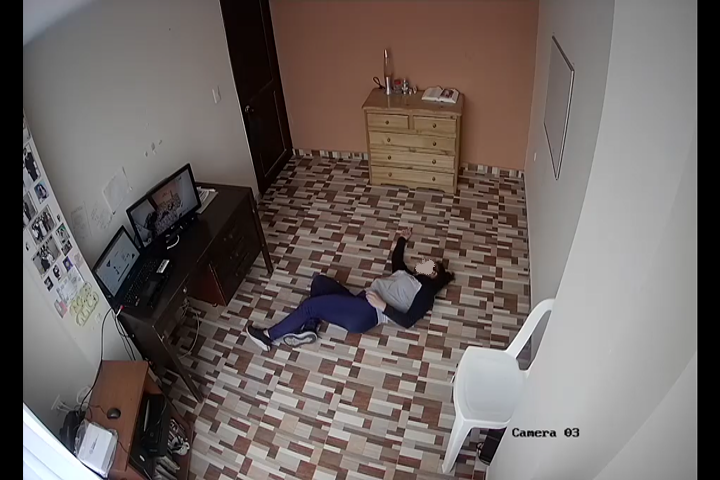
\includegraphics[width=0.45\textwidth]{Figures/datasets_examples/cauca1.png}
    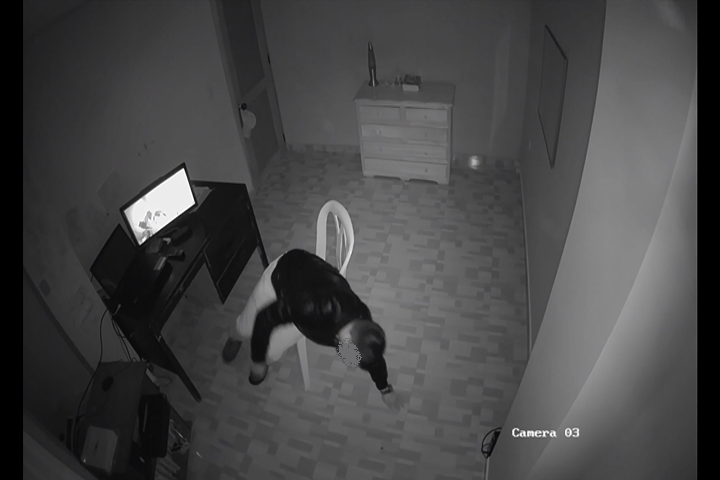
\includegraphics[width=0.45\textwidth]{Figures/datasets_examples/cauca2.png}
    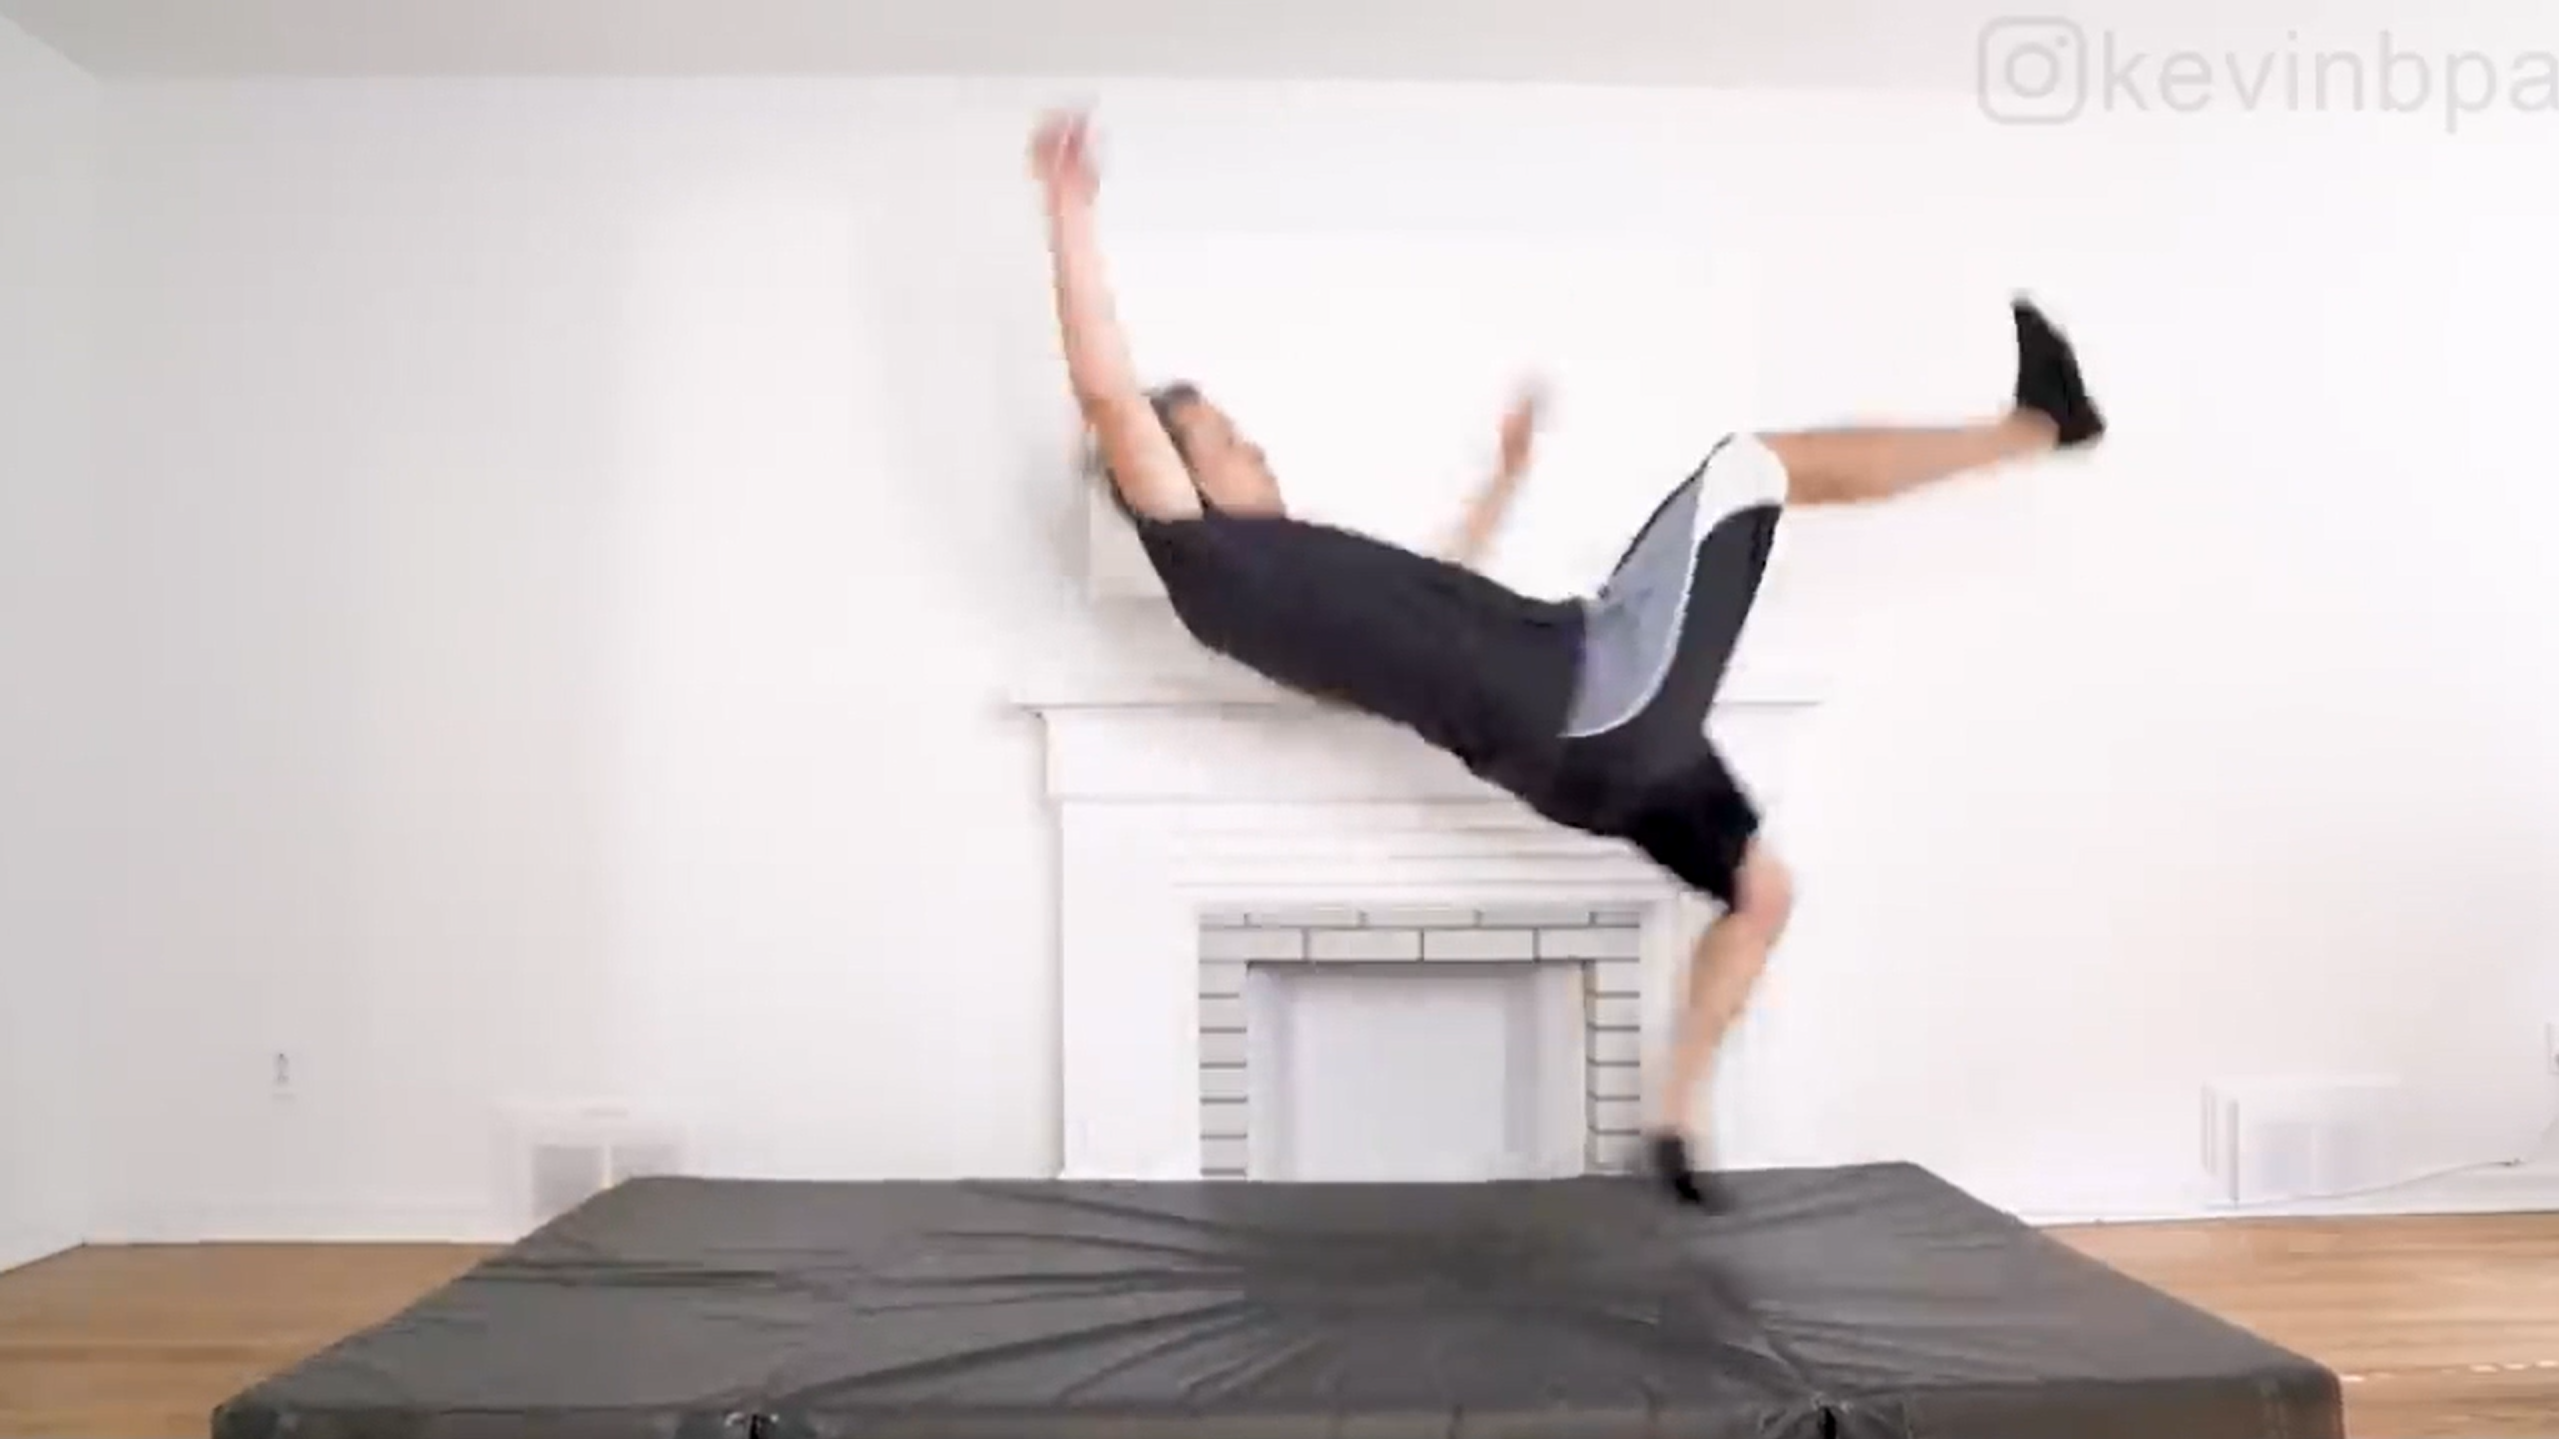
\includegraphics[width=0.45\textwidth]{Figures/datasets_examples/fifty1.png}
    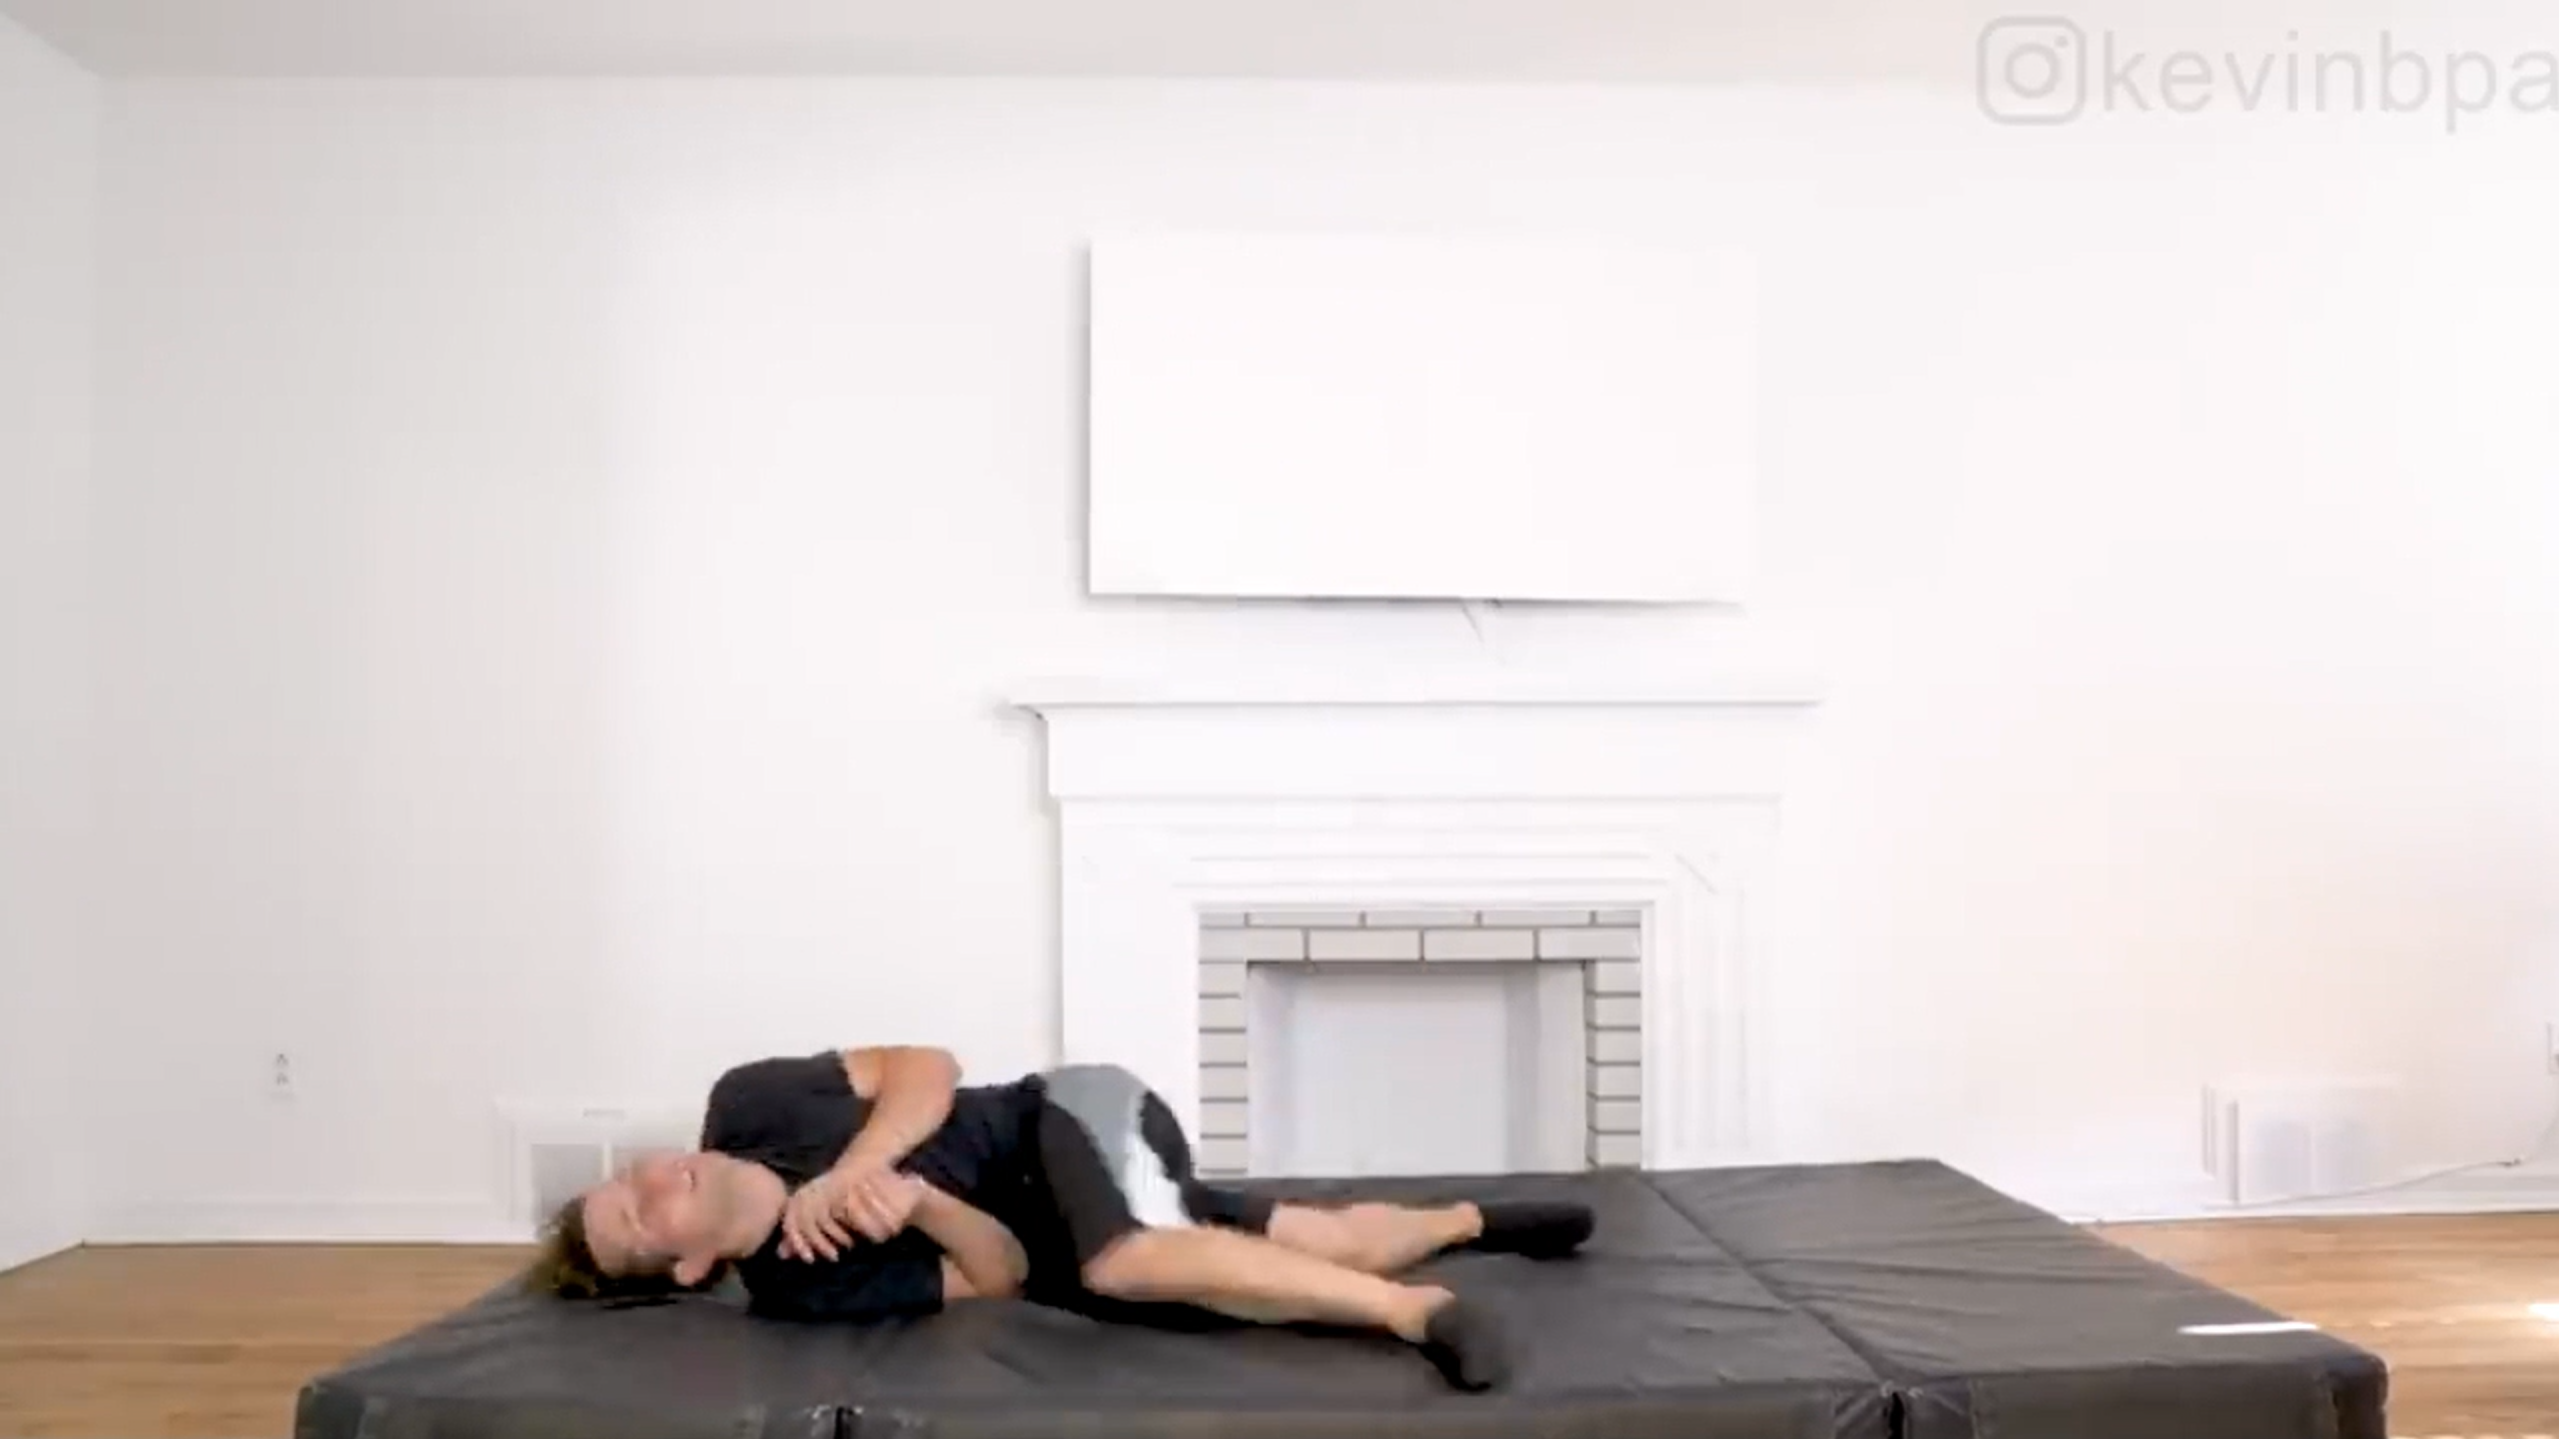
\includegraphics[width=0.45\textwidth]{Figures/datasets_examples/fifty2.png}
    \caption{Příkladové snímky z datasetů CAUCAFall (nahoře) a 50 Ways to Fall (dole).}
    \label{fig:datasets_examples}
\end{figure}

V obou případech se jedná o videa vždy jedné osoby. To proto, že použijeme
detekční algoritmus již natrénovaný na videích s více osobami, a náš
klasifikační algoritmus bude zpracovávat každou osobu zvlášť. Práce s více
osobami tak bude úlohou výsledného detektoru, nikoliv trénované klasifikační
sítě.

Oba datasety jsme rozdělili do tří sad: trénovací, validační a testovací. Rozděleny byly v tomto poměru: trénovací sada 70\%, validační sada 15\% a testovací sada 15\%. Trénovací a validační sada budou použity v procesu trénování - trénovací pro výpočet ztráty a úpravu vah, validační pro průběžné ověřování výkonu, a testovací sada bude na konci použitá pro otestování jednak klasifikačního algoritmu, jednak celkového řešení.

\section{Třídy a jejich anotace}
Pro videa byly vytvořeny anotace aktuální třídy pózy. Tato anotace není pro
každý snímek, ale pouze při změně definuje časovou značku a následující třídu.

V anotacích jsme použili 3 třídy, ty odpovídají třem různým třídám pózy, které
nás mohou zajímat - \textit{normální}, kdy osoba např. chodí, sedí nebo stojí,
\textit{padá} - přechodný stav padání, definován od započatí pohybu směrem
dolů, a \textit{upadl} - definován od momentu, kdy se dotkl země trupem nebo
všemi končetinami.

%todo
Pro náš model obecně potřebujeme jenom dvě třídy - \textit{normální} a
\textit{upadl}. Skript tvořící trénovací data proto považuje třídu
\textit{padá} za třídu \textit{normální}. Nicméně později budeme pro náš model
experimentovat i se třídou \textit{padá}, která může síti pomoct hlouběji
pochopit problematiku a přesněji rozeznat některé situace, zejména pak v
případě využití rekurentních neuronových sítí.

\section{Příprava trénovacích dat pro klasifikační algoritmus}

Dále byl vytvořen skript, který prošel každé video z trénovacích datasetů a
vytvořil trénovací data pro naši klasifikační síť. Ty obsahují pro každý snímek
detekované klíčové body (jako vstup) a aktuální třídu (jako požadovaný výstup).
Pro detekci klíčových bodů byl použit vybraný model pro detekci pózy. Výběr
modelu je popsán v následující kapitole. Na použitém modelu by teoreticky
nemuselo záležet (pokud detekuje stejné typy klíčových bodů), je ale lepší
použít ve výsledném programu stejný model jako pro trénovací data. Modely se
totiž můžou v některých situacích chovat trochu jinak (např. okluze) a náš
model by tak dostával v praxi jiná data, než pro jaké byl natrénován.

Jelikož pro rekurentní neuronové sítě potřebujeme sekvenci snímků, musí být
trénovací data ještě zpracována. To ale bude již součastí samotného trénovacího
skriptu, jelikož se konečná podoba dat může lišit hlavně délkou sekvencí, dále
ale taky dodatečným rozšířením o sekvence vynechávající určité množství snímků,
což simuluje menší snímkovou frekvenci (FPS).

\endinput